
Dans le cadre de ce stage, les données que l'on traite sont des données du secteur de l'énergie, et plus particulièrement des données de production électrique. On dispose ainsi de plusieurs éoliennes identifiées par le tag "id\_[identifiant de l'éolienne]" dont l'énergie produite est mesurée toutes les demies heures, et ce pendant 4 ans (de de 2014 à 2017).
Cette énergie produite est dénommée la courbe de charge (que l'on abbrégera par \textbf{CDC} par la suite). Il est cependant plus utile de s'intéresser au facteur de charge (ou \textbf{FDC}) qui est défini comme
$\displaystyle\textsf{Facteur de Charge} = \frac{\textsf{Courbe de Charge}}{\textsf{Puissance Installée}}$.
On en déduit que \textbf{FDC} doit nécessairement être compris entre 0 et 1. C'est entre autre aussi une manière de détecter des anomalies et données atypiques comme la surproduction d'énergie par rapport à ce qui était attendu de la part d'un parc éolien ou encore un défaut de capteur (tension / intensité, ...) qui mesure la courbe de charge.

% TODO ⚠️✏️
% données éoliennes : indépendantes
% ⇒ parcs éoliens différents : géographiquement éloignés
% données photovoltaïques : données dépendantes
% montrer différence en pratique entre le cas dépendant et indépendant}

\begin{figure}[H]
	\centering
	période : Première semaine de Juin 2015

	\scalebox{0.95}{
		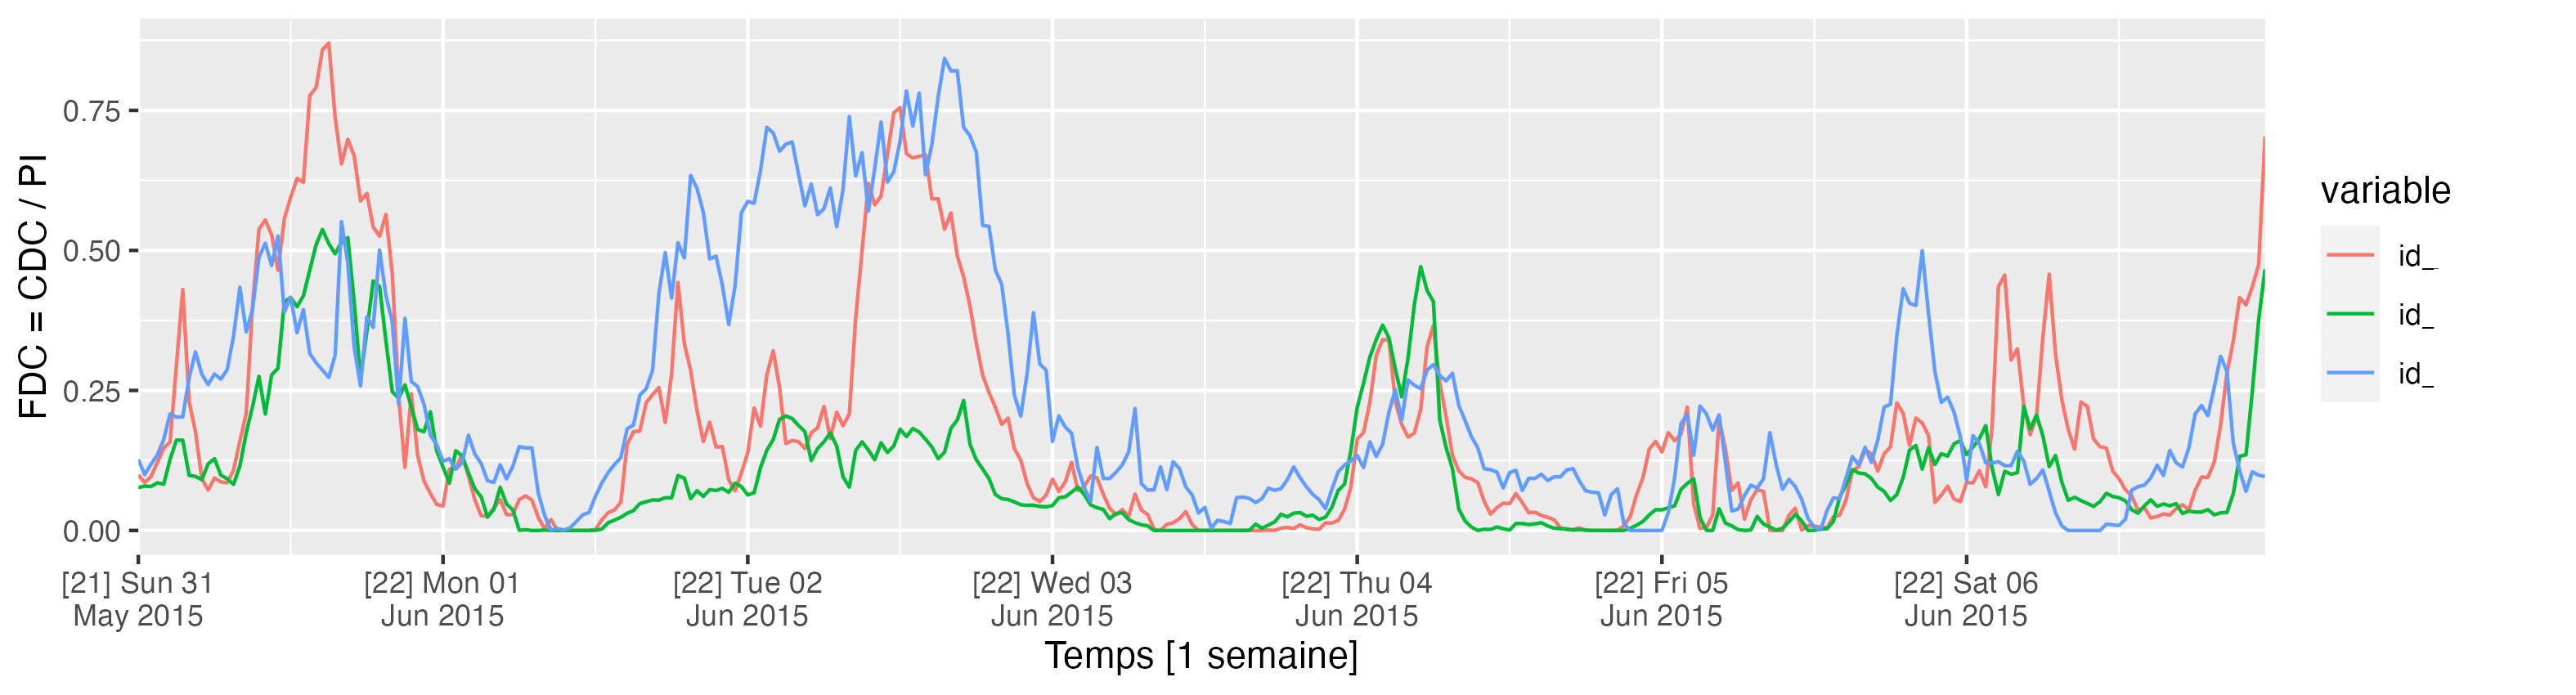
\includegraphics[width=0.75\textwidth]{Images/motivation/test__slice_graph__2015__id_1_2_3__week_1.jpg}
	}

	période : Juillet 2015

	\scalebox{0.95}{
		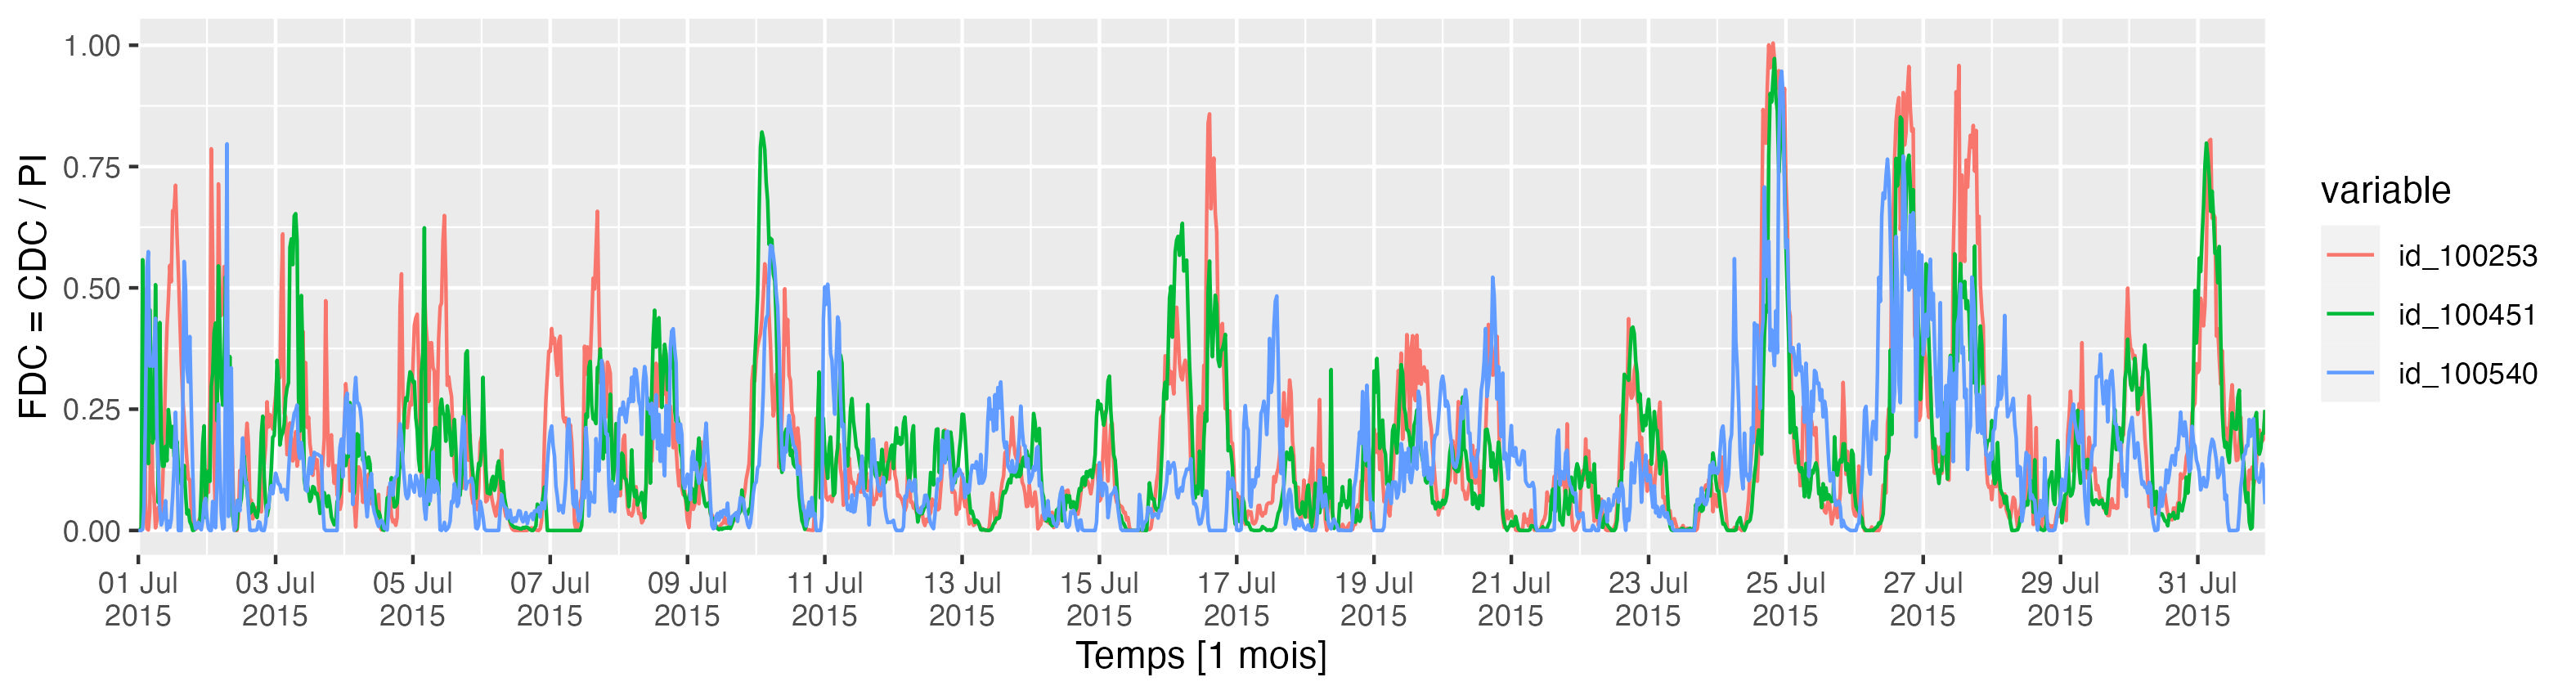
\includegraphics[width=0.75\textwidth]{Images/motivation/test__slice_graph__2015_07__id_1_2_3.jpg}
	}
	\caption{Courbes de charges éoliennes sur 3 premiers parcs éoliens}
	\label{fig:courbes_de_charge}
\end{figure}

Ainsi, les données qui sont traitées dans le cadre de ce stage sont, entre autres, des courbes de charge éoliennes observées chaque demie-heure. Le schéma d’observation est donc le 'common-design'. C'est-à-dire que les temps d'observations sont ici déterministes à intervalle de temps fixe.